\documentclass[ngerman,inputenc]{beamer}

\usepackage{amsmath, amssymb}
\usepackage{appendix}
\usepackage{pstricks}
\usepackage[utf8]{inputenc}
\usepackage{tikz}

\usepackage{graphicx} %package to manage images
\graphicspath{{images/}}

\definecolor{darkblue}{cmyk}{1.0,0.3,0,0.5}
\definecolor{darkred}{cmyk}{0.25,1,0.1,0.1}
\definecolor{uniblau}{cmyk}{1.0,0.7,0.1,0.6}
\definecolor{unihellblau}{cmyk}{0.2,0.14,0,0}
\definecolor{unihellhellblau}{cmyk}{0.05,0.035,0,0}
\definecolor{darkerblue}{cmyk}{1.0,0.3,0,0.7}

\setbeamertemplate{headline}{
\setbeamercolor{author in head/foot}{fg=white,bg=uniblau!80}
 \hbox{%
  \begin{beamercolorbox}[wd=\paperwidth,ht=2.25ex,dp=1ex,left]{author in head/foot}%
    \usebeamerfont{author in head/foot} \hspace{3pt} \insertsection%
  \end{beamercolorbox}
  }
}

\setbeamertemplate{frametitle}
{
    \setbeamercolor{frametitle}{fg=white,bg=uniblau}
    \vspace{-0.1em}
  \begin{beamercolorbox}[wd=\paperwidth,ht=3ex,dp=2ex,left]{frametitle}%
    \usebeamerfont{frametitle}\hspace{0.7em} \textbf{\insertframetitle}%
  \end{beamercolorbox}%
}

\setbeamertemplate{footline}
{
  \leavevmode%
   \hspace{-1em}
  \hbox{%
    \setbeamercolor{author in head/foot}{fg=white,bg=uniblau!60}
  \begin{beamercolorbox}[wd=.42\paperwidth,ht=2.25ex,dp=1	ex,center]{author in head/foot}%
    \usebeamerfont{author in head/foot}\insertshortauthor~~(\insertshortinstitute)
  \end{beamercolorbox}%
  \hspace{-1em}
\setbeamercolor{title in head/foot}{fg=white,bg=uniblau!80}
  \begin{beamercolorbox}[wd=.35\paperwidth,ht=2.25ex,dp=1ex,center]{title in head/foot}%
    \usebeamerfont{title in head/foot}\insertshorttitle
  \end{beamercolorbox}%
  \hspace{-1em}
  \setbeamercolor{date in head/foot}{fg=white,bg=uniblau}
  \begin{beamercolorbox}[wd=.25\paperwidth,ht=2.25ex,dp=1ex,right]{date in head/foot}%
    \usebeamerfont{date in head/foot}\insertshortdate{}\hspace*{1em}
    \insertframenumber{} /
    \inserttotalframenumber\hspace*{2ex}
  \end{beamercolorbox}}%
  \vskip0pt%
}

\let\ueberschrift=\frametitle
\renewcommand\frametitle[1]{%
  \ueberschrift{
  \rput[l](0,0){#1}
  }
}

\usecolortheme[named=uniblau]{structure}

\title[Airbnb Oslo]{Price Predictions on Airbnb Accomodations in Oslo, Norway}
\date{21.02.2022}
\author[Freitag, Beck]{Marei Freitag, Joel Beck}
\institute[University Göttingen]{Georg-August-University of Göttingen}

% display TOC before every section and subsection without duplicates
% https://stackoverflow.com/questions/2795478/latex-beamer-prevent-showing-the-toc-at-one-occasion

\RequirePackage{ifthen}
\newboolean{sectiontoc}
\setboolean{sectiontoc}{true} % default to true

\AtBeginSection[]
{
  \ifthenelse{\boolean{sectiontoc}}{
  \begin{frame}
    \frametitle{Table of Contents}
    \tableofcontents[currentsection, currentsubsection, subsubsectionstyle={show/show/shaded/shaded}]
  \end{frame}
  }
}

\AtBeginSubsection[]
{
  \begin{frame}
    \frametitle{Table of Contents}
    \tableofcontents[currentsection, currentsubsection, subsubsectionstyle={show/show/shaded/shaded}]
  \end{frame}
}

\newcommand{\toclesssection}[1]{
  \setboolean{sectiontoc}{false}
  \section{#1}
  \setboolean{sectiontoc}{true}
}


\begin{document}

\begin{frame}
  \titlepage
\end{frame}


\begin{frame}
  \frametitle{Table of Contents}
  \tableofcontents
\end{frame}

%%%%%%%%%%%%%%%%%%%%%%%%% Kapteil 1 %%%%%%%%%%%%%%%%%%%%%%%%%

\toclesssection{1. Introduction}

\begin{frame}{Introduction}

  Aims of this work:
  \begin{itemize}
    \item Establish a deep learning approach to predict the price of an accomodation per night
    \item Focus on explainability and interpretability
  \end{itemize}
  \hspace{12pt}

  $\rightarrow$ Underlying Data: provided by Airbnb, contains various information about the listings in Oslo, Norway

\end{frame}


%%%%%%%%%%%%%%%%%%%%%%%%% Kapteil 2: Methods %%%%%%%%%%%%%%%%%%%%%%%%%

\toclesssection{2. Methods}

%%% Data Preprocessing %%%
\subsection{2.1 Preprocessing}

\subsubsection{Feature Engineering}

\begin{frame}{Feature Engineering: Images}

  \begin{itemize}
    \item Use transfer learning on a pretrained CNN (ResNet18)
    \item But have to be sure, the CNN is able to generalize: added Fully Connected Network at the end containing three layers and \texttt{ReLU} activation functions
    \item Also implemented CNN manually as a benchmark model to compare the results
  \end{itemize}

  \hspace{5pt}

  Results:
  \begin{itemize}
    \item pretrained \texttt{ResNet18} achieved a Mean Absolute Error of $579$ NOK (approx. $58$ Euros) on the Validation Set
    \item But \emph{correlation} of the CNN predictions with the true price was $0.41$
  \end{itemize}

\end{frame}

\begin{frame}{Image Predictions}

  Beispiel Bilder der Predictions!
  % COMMENT: 2 x 4 wäre gut!
  \begin{figure}[H]
    \centering
    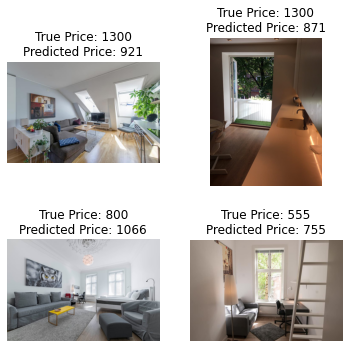
\includegraphics[width=6cm]{cnn_examples_small.png}
    \caption{CNN example predictions}
  \end{figure}


\end{frame}


\begin{frame}{Feature Engineering: Reviews}
  % Language and Sentiment
  \begin{itemize}
    \item Language: Detect language of each review
    \item Sentiment analysis: Get the sentiment of each review
  \end{itemize}

  \hspace{5pt}

  New Features per listing:
  \begin{itemize}
    \item[1.] Number of reviews
    \item[2.] Median review length
    \item[3.] Number of different languages of the reviews as well as a list of the different languages
    \item[4.] Fraction of Norwegian and English reviews
    \item[5.] Ratio of negative reviews to the total number of reviews
  \end{itemize}

\end{frame}

\begin{frame}{Feature Engineering: Reviews}

  % Wordcloud
  \begin{figure}[t]
    \centering
    \begin{minipage}{6.7cm}
      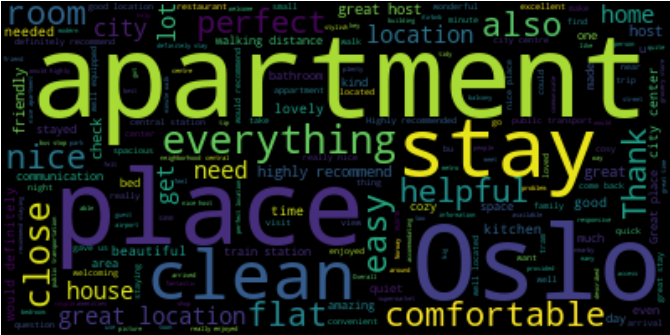
\includegraphics[width=\columnwidth]{wordcloud_eng.png}
    \end{minipage}
    \begin{minipage}{6.7cm}
      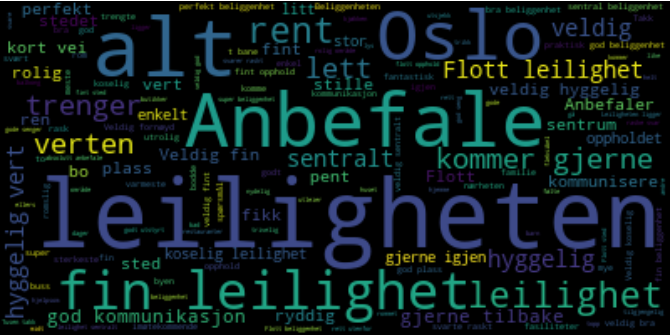
\includegraphics[width=\columnwidth]{wordcloud_nor.png}
    \end{minipage}
    \caption{Wordclouds in English and Norwegian}
    \label{fig:wordclouds}
  \end{figure}

\end{frame}


\subsubsection{Feature Selection}

\begin{frame}{Feature Selection \& Data Cleaning}

  Feature Selection:
  \begin{itemize}
    \item[1.] Manually selected features based on three criteria
    \item[2.] Analyzed results of different feature selection algorithms
  \end{itemize}

  \hspace{5pt}

  Data Cleaning:
  \begin{itemize}
    \item Converting data types
    \item Splitting text-based variables into more convenient numeric or boolean features
    \item Aggregating rare categories of categorical variables into one larger \emph{Other} group to stabilize estimation
    \item One-Hot Encoding of categorial variables and standardization of numerical variables
  \end{itemize}

\end{frame}


%%% Models %%%

\subsection{2.2 Models}

\subsubsection{Classical Models}

\begin{frame}{Classical Models}
  % In order to get some insights, we selected four classical Machine Learning models of varying complexity from the \texttt{scikit-learn} library \citep{pedregosa2011} to serve as benchmark models for our custom Neural Net.

  \begin{itemize}
    \item[1.] \textbf{Linear Regression}: simple, well understood in terms of underlying theory and highly interpretable.
    \item[2.] \textbf{Ridge Regression}: still very interpretable with a closed form analytical solution, adds one hyperparameter to the equation
    \item[3.] \textbf{Random Forest}: very flexible model with many hyperparameters determining e.g. the number of regression trees and the tree depth. Can be applied to many contexts and often works 'out of the box'.
    \item[4.] \textbf{Histogram-Based Gradient Boosting}: modern and fast tree-based gradient boosting algorithm.Comes with a large number of tunable hyperparameters, some of them similar to the Random Forest parameters, some of them more specific to the \emph{Boosting} instead of the \emph{Bagging} approach such as the learning rate.
      %Similar to the very popular \href{https://xgboost.readthedocs.io/en/stable/}{XGBoost} \citep{chen2016} and \href{https://lightgbm.readthedocs.io/en/latest/}{LightGBM} \citep{ke2017} implementations that regularly outperform deep Neural Networks in Kaggle competitions on tabular data.
  \end{itemize}

\end{frame}


\subsubsection{Neural Network}

\begin{frame}{Neural Network}

  explain Hyperparameter and Architecture

\end{frame}

\begin{frame}{Model Architecture}

  \begin{figure}[t]
    \centering
    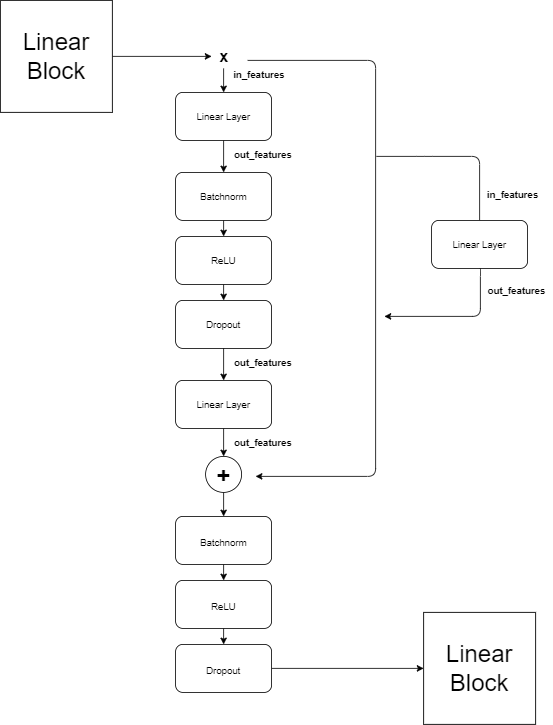
\includegraphics[width=0.4\textwidth]{mlp_architecture.png}
    \caption{Architecture of each Block in the Fully Connected Neural Network}
    \label{fig:linear-block}
  \end{figure}

\end{frame}




%%%%%%%%%%%%%%%%%%%%%%%%% Kapteil 3: Results %%%%%%%%%%%%%%%%%%%%%%%%%

\section{3. Results}

\begin{frame}{Test - Slide 1}

\end{frame}

%%%%%%%%%%%%%%%%%%%%%%%%% Kapteil 4: Conclusion %%%%%%%%%%%%%%%%%%%%%%%%%

\section{4. Conclusion}

\begin{frame}{Test - Slide 2}

\end{frame}


\begin{frame}

  \begin{center}
    \LARGE{\textbf{Thanks for listening!}}\\[10mm]
    \large{Questions?}
  \end{center}

\end{frame}


\end{document}
%
